\documentclass{article}
\usepackage{listings}
\usepackage{verbatim}
\lstset{
    frame=single,
    breaklines=true
}
\usepackage{geometry}
\geometry{margin=1in}		%set margins

\usepackage{graphicx}		%need for images
\usepackage{float}			%need for arranging graphics and tables


\title{ECG 782 HW 4}
\date{2015-10-15}
\author{Carlo Lopez-Tello}

\begin{comment}

how to paste code

\lstinputlisting[language=Octave]{Q1/histEqualize.m}

how to paste image

\begin{figure}[H]
	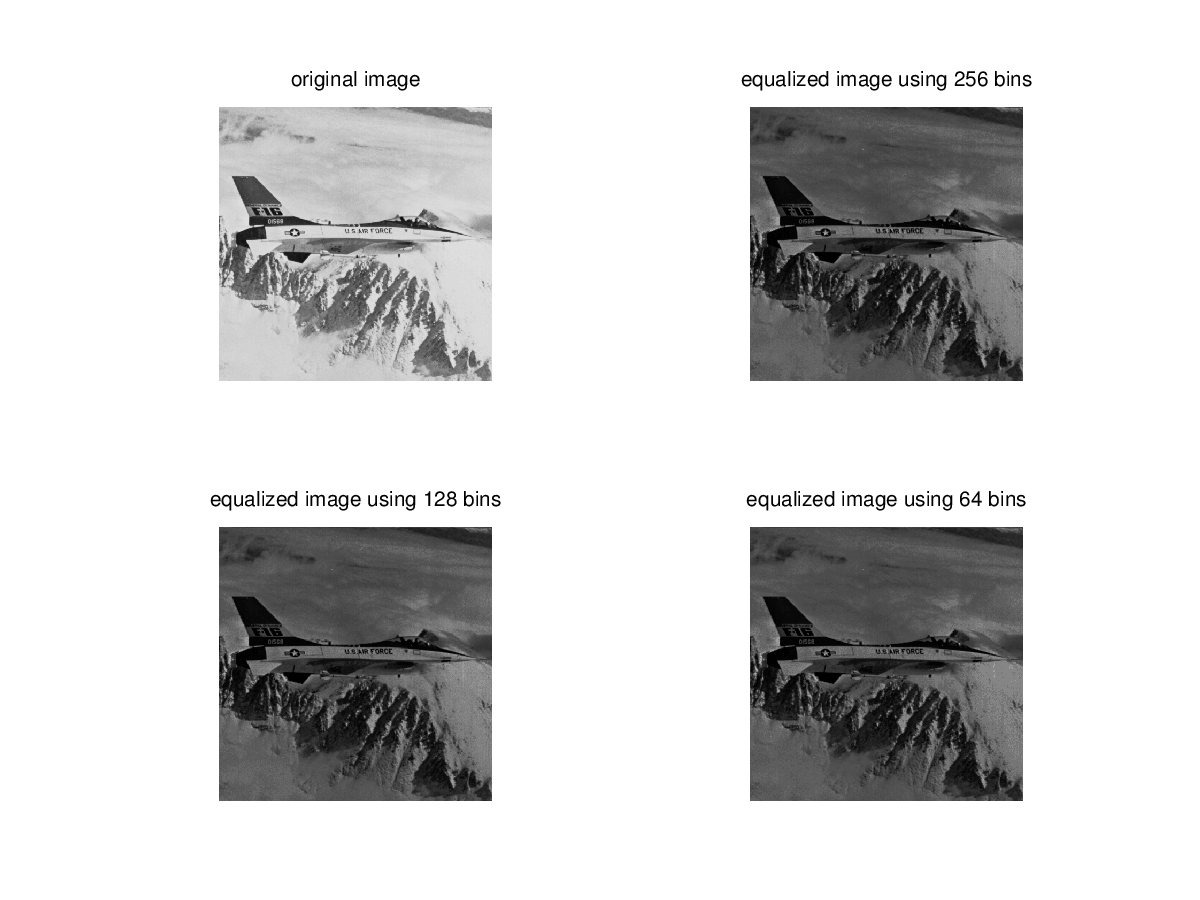
\includegraphics[width=\linewidth]{Q1/outputImages.png}
	\caption{equalized images}
\end{figure}

how to start newpage

\newpage

how to make table

\begin{table}[H]
	\centering
	\begin{tabular}{ c | c | c }
		filter & MSE & PSNR \\
		none & 72.0 & 29.6 \\
		3x3 mean filter & 32.9 & 33.0 \\
		5x5 mean filter & 36.7 & 32.5 \\
		3x3 median filter & 37.2 & 32.4 \\
		5x5 median filter & 36.2 & 32.5 \\
	\end{tabular}
	\caption{SNR and PSNR after filtering the noisy image}
\end{table}
	

\end{comment}
\begin{document}
\maketitle
	\newpage
	\section{Problem 10.49}
	
	\subsection{Maximum exposure time}
	We are given the dimensions of the image 256 by 256 pixels. We now that the bullet takes up 10 percent of the width of the image and that the bullet is 3 cm long. This implies that the image is 30 cm by 30 cm. Thus, each pixel is .12 cm by .12 cm. The exposure time has to be fast enough so that the bullet can only move .12 cm or 1 pixel. We can calculate the exposure time using \(.12 cm = speed(exposure)\). We know the maximum speed of the bullet is 900 m/s so we can calculate the exposure time to be 1.33 us.
	
	\subsection{Minimum FPS}
	We want the time between frames to be fast enough so that the bullet is always captured in two consecutive frames. In other words the bullet cannot move more than half the width of the image between frames. The problem with this limit is that we can have half a bullet in one frame if we capture exactly as the bullet hits the midpoint of the image. Thus the bullet cannot travel more than half the width minus the lenght of the bullet minus the two pixels from motion blur \(128 - 26 - 2 = pixels\). We can convert 100 pixels to the actual distance of 12 cm. Thus, the maximum distance that a bullet can move between frames is 12 cm. We can calculate the framerate using \(12 cm(FPS) = speed\). For a bullet travelling at the max speed of 900 m/s, the framerate should be higher than 7500 FPS.
	
	\subsection{Bullet Segmentation}
	Assuming we have control over the scene. Meaning that we have constant illumination and background. We can use simple frame differencing between the recording and an image of the background.
	
	\subsection{Calculationg bullet speed}
	We can easily calculate the speed of the bullet if we know how many pixels it moved between frames. In order to do this we need to find a point corresponding to the same part of the bullet in both images. We can use a corner of the bullet and try to match it to the next frame. Once we know the number of pixel the bullet moved we can calculate the distance and divide it by the time between frames.
	
	
	\section{Background Subtraction}
	
	\subsection{simple frame differencing}
	\begin{figure}[H]
		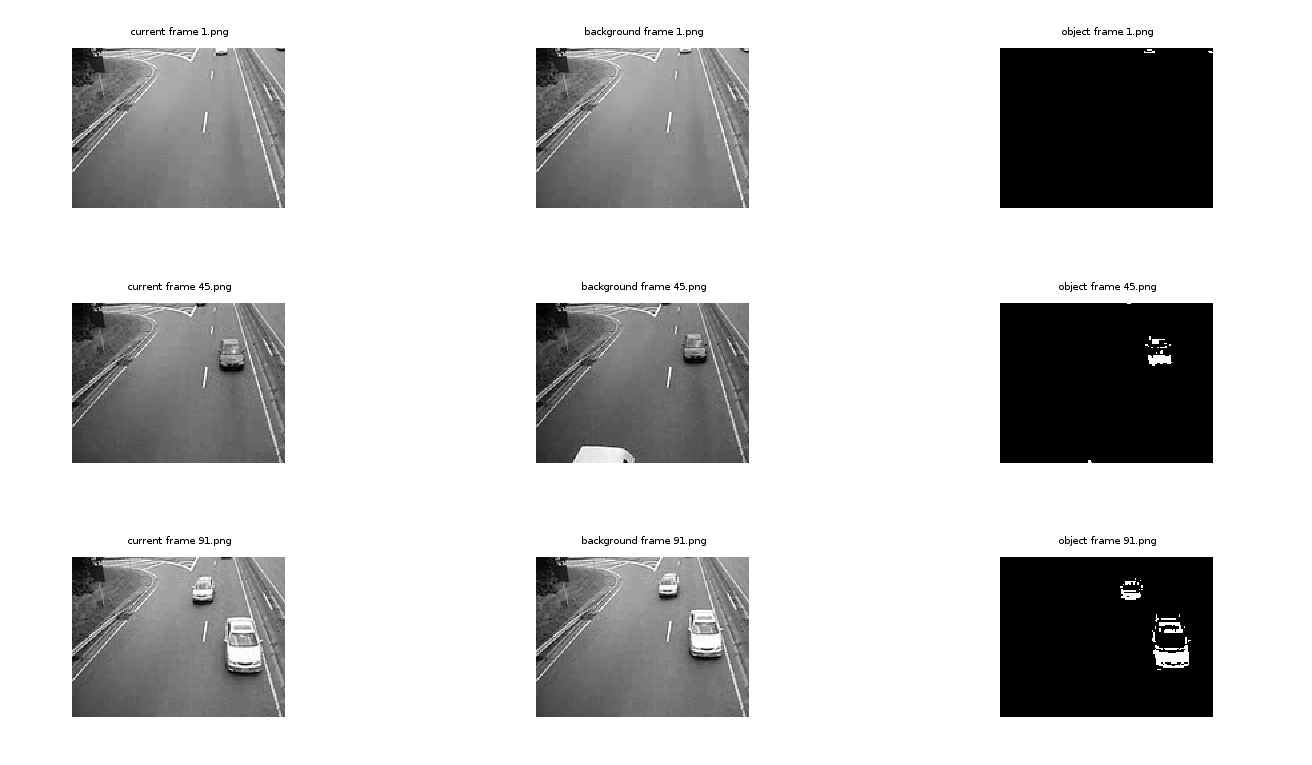
\includegraphics[width=\linewidth]{Q2/partA/partA.png}
		\caption{simple frame differencing}
	\end{figure}
	
	\newpage
	\subsection{static background}
	\begin{figure}[H]
		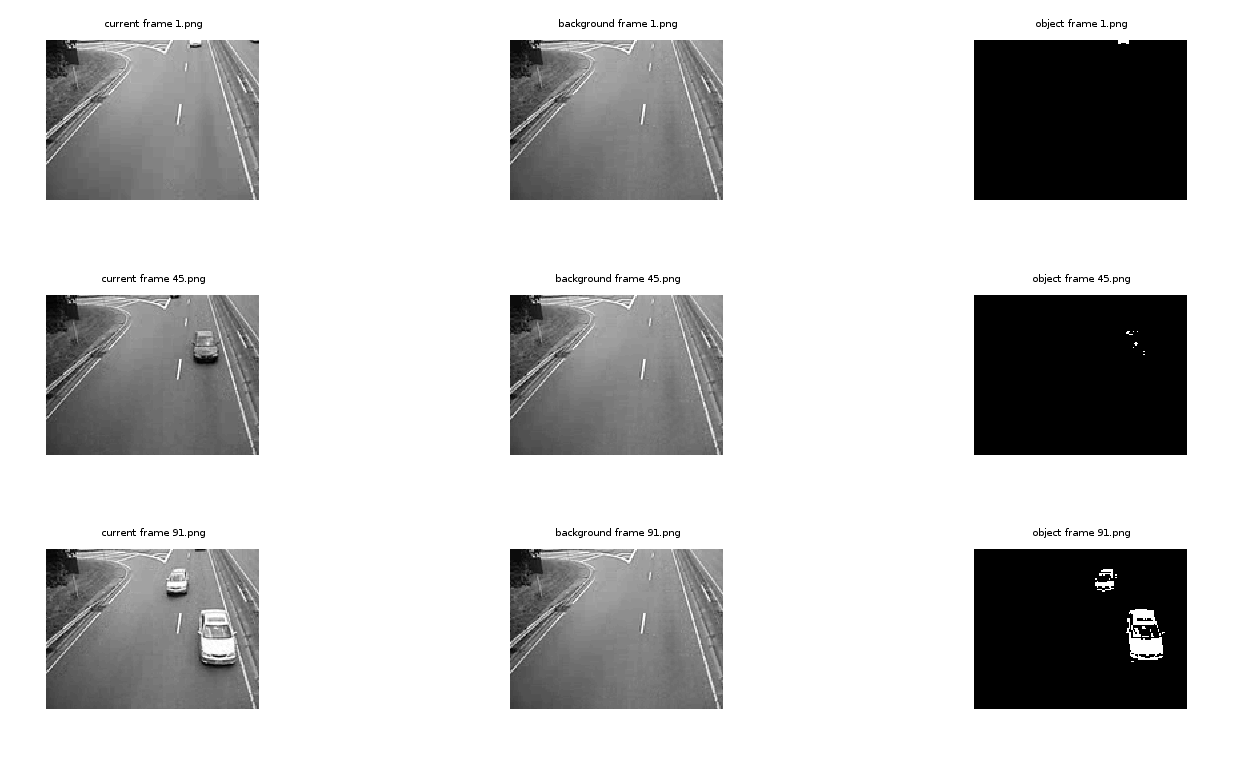
\includegraphics[width=\linewidth]{Q2/partB/partB.png}
		\caption{static background}
	\end{figure}
	
	\subsection{static average background}
	\begin{figure}[H]
		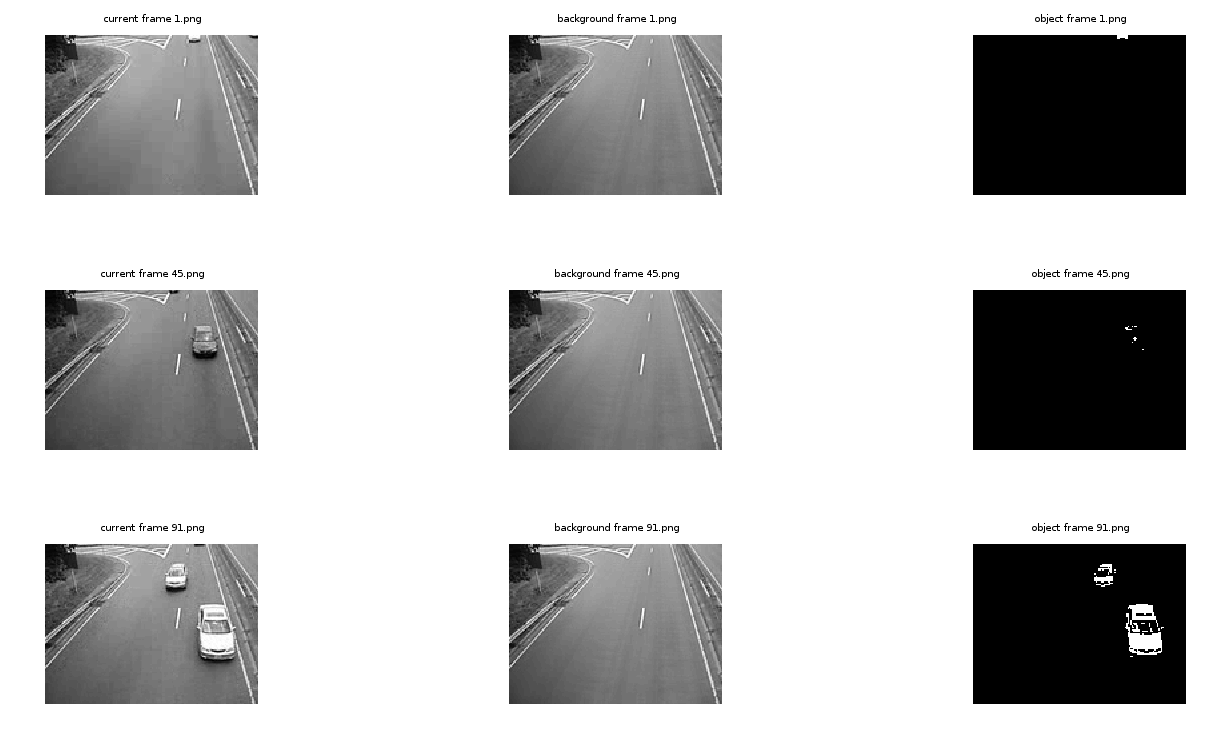
\includegraphics[width=\linewidth]{Q2/partC/partC.png}
		\caption{static average background}
	\end{figure}
	
	\subsection{adaptive background}
	\begin{figure}[H]
		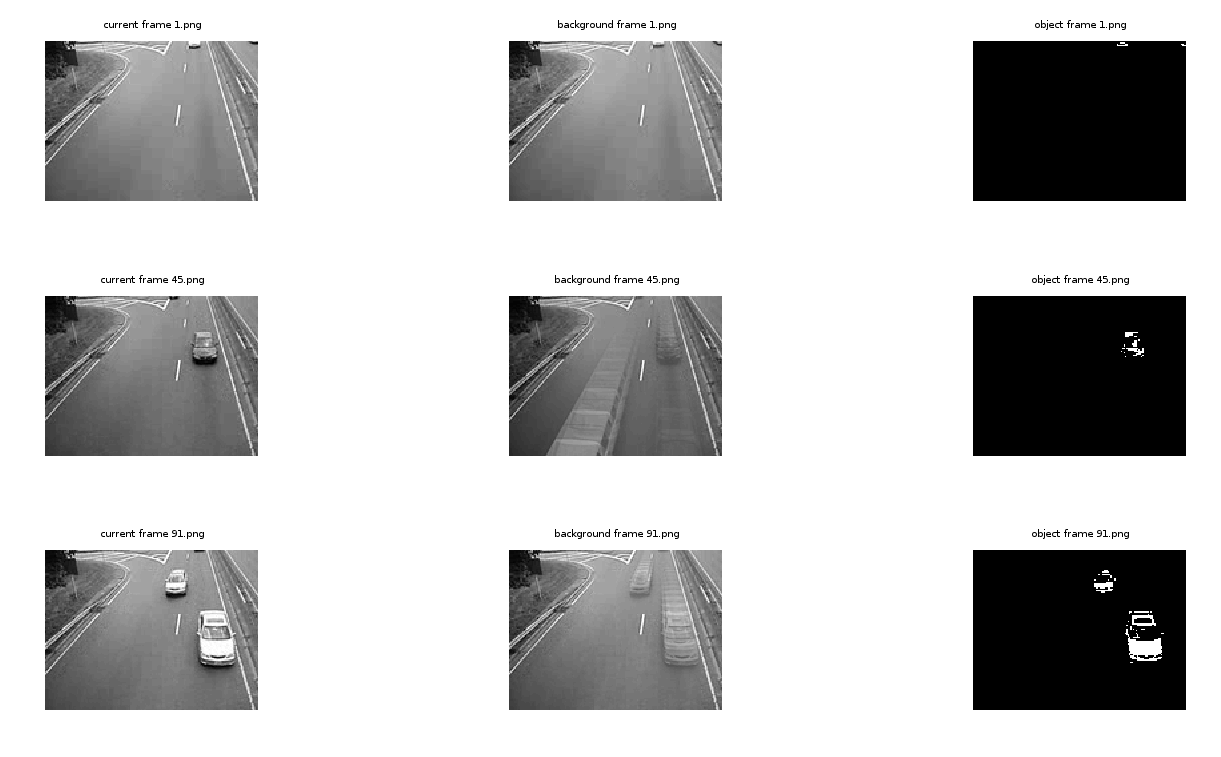
\includegraphics[width=\linewidth]{Q2/partD/partD.png}
		\caption{adaptive background}
	\end{figure}
	
	\newpage
	\section{Gaussian Mixture Model}
	
	\subsection{foreground extraction}
	\begin{figure}[H]
		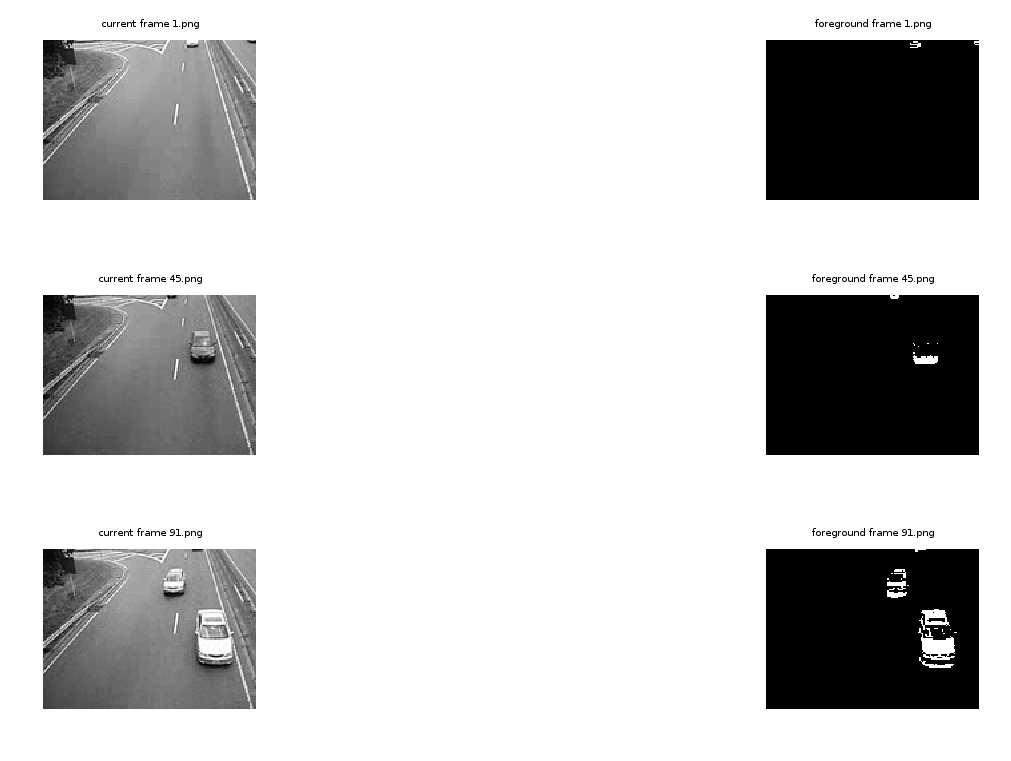
\includegraphics[width=\linewidth]{Q3/partA/partA.png}
		\caption{adaptive background}
	\end{figure}
	
	\subsection{clean foreground}
	\begin{figure}[H]
		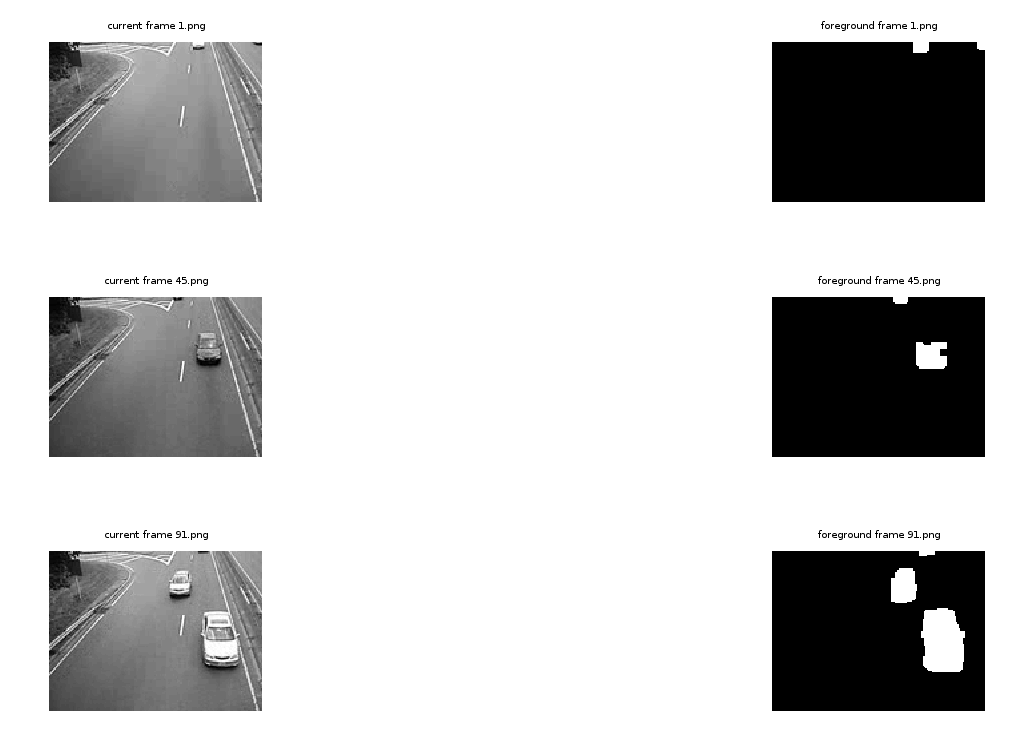
\includegraphics[width=\linewidth]{Q3/partB/partB.png}
		\caption{adaptive background}
	\end{figure}
	
	\subsection{vehicle detection}
	\begin{figure}[H]
		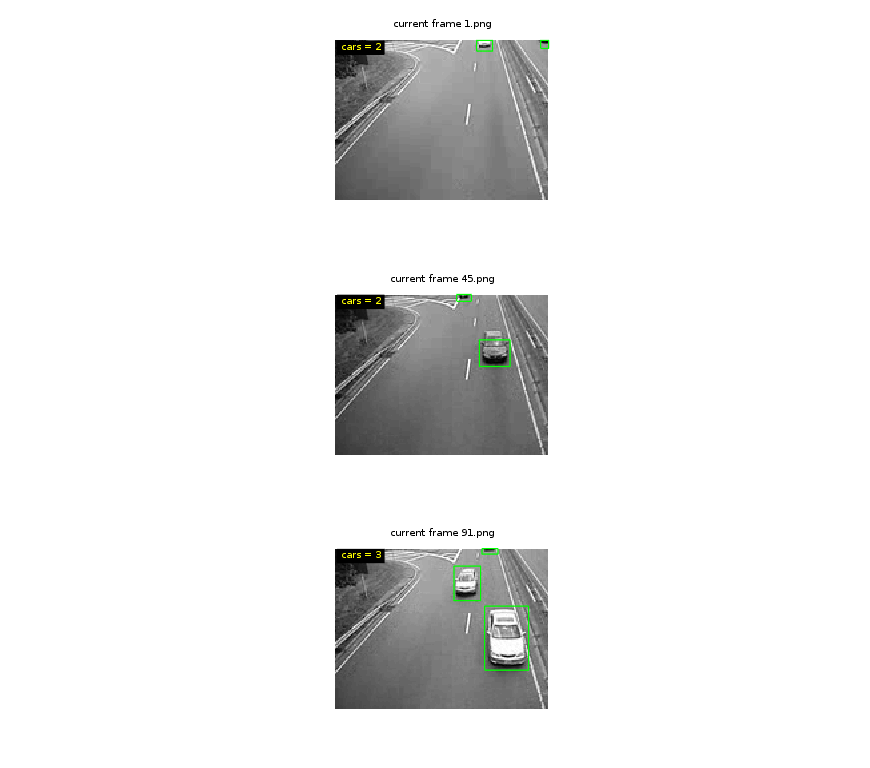
\includegraphics[width=\linewidth]{Q3/partC/partC.png}
		\caption{adaptive background}
	\end{figure}
	
	\begin{comment}
	\newpage
	\section{Code}
	
	Part 5.A
	\lstinputlisting[language=Octave]{Q5/gradkernel.m}
	\newpage
	
	Part 5.B
	\lstinputlisting[language=Octave]{Q5/canny.m}
	\newpage
	
	Part 5.C
	\lstinputlisting[language=Octave]{Q5/partC.m}
	\newpage
	
	Part 5.D
	\lstinputlisting[language=Octave]{Q5/partD.m}
	\newpage
	
	Utility Code
	\lstinputlisting[language=Octave]{Q5/normalizeImage.m}
	\newpage
	
	Part 5.A
	\lstinputlisting[language=Octave]{Q6/partA.m}
	\newpage
	
	Part 5.B
	\lstinputlisting[language=Octave]{Q6/houghCircle.m}
	\newpage
	
	\lstinputlisting[language=Octave]{Q6/partB.m}
	\newpage
	
	\end{comment}
	
	
	
	
	
	
\end{document}
